\chapter{Roadmap for connectivity enhancement and Flagship Projects}

\tab Based on all the issues presented and the solutions proposed in the previous chapters, this chapter summarizes the key development areas for the enhancement of ASEAN connectivity and resilience. ASEAN countries being divided in two categories, insular and continental, it is necessary to take into account their relatives specificities.

Therefore, this chapter differentiates between land connectivity and ocean connectivity, and proposes recommendations aiming at their enhancement. For each of them, after stating precise targets, we recommend specific actions which should be carried out to achieve those targets.

\section{Better Land Connectivity} \label{land}

\tab More than half of ASEAN countries --- in alphabetical order, Cambodia, Lao P.D.R., Malaysia (partially), Myanmar, Singapore, Thailand, and Vietnam --- are continental. Therefore, enhancing land connectivity is a great priority for ASEAN.

\begin{figure}[H]
\begin{center}
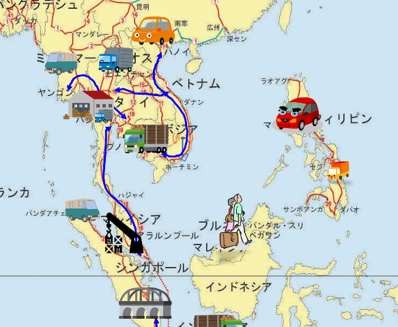
\includegraphics[width = 0.8\linewidth]{Figures/land_connect.png}
\end{center}
\caption{Improved land connectivity with SGT}
\label{land_connect}
\end{figure}

\subsection{Targets}

\begin{enumerate}

\item Smoother and safer transport, logistics, and people flow 

\begin{itemize}
\item Drastic cost reduction and accident reduction for mobility
\end{itemize}

\item Better and secure management of transportation (e.g. road pricing, cargo management, people mobility management)

\begin{itemize}
\item Better security and management, reduction of GHGs
\end{itemize}

\item Accelerating implementation of  autonomous vehicles, automation in transport, logistics, construction, agriculture/forestry etc.

\begin{itemize}
\item Advanced/leading technologies and implementation
\end{itemize}

\item Providing advanced positioning services for safer mobility

\begin{itemize}
\item World-first services for safer and securer mobility
\end{itemize}

\end{enumerate}

\subsection{Actions}

\begin{enumerate}

\item Develop incubation centers of advanced positioning services and applications

\begin{enumerate}
\item High precision, authentication (anti-spoofing)
\item Support of industrial development and business creation.
\item Model case; GNSS incubation center (GISTDA, Thailand)
\end{enumerate}

\item Establish connected networks of GNSS base stations

\begin{enumerate}
\item Common location basis of ASEAN for better consistency and accuracy
\item High-precision mapping, autonomous vehicle (logistics, public transport) and machines (logistics, agriculture, construction etc.), crust monitoring
\item Enhancing NSDI (National Spatial Data Infrastructure) to better geospatial data dissemination and integration
\end{enumerate}

\item Provide world-first advanced positioning services

\begin{enumerate}
\item Free high precision, authentication service with QZSS
\item Accelerate social implementation: Road pricing, Illegal vehicle detection, Secure logistics
\end{enumerate}

\item Develop data sharing infrastructure and human resource development facility

\begin{enumerate}
\item Logistics, transportation, people flow, autonomous vehicle etc.
\item Incubation of data experts serving better data usage and management
\end{enumerate}

\end{enumerate}


\section{Better Sea Connectivity} \label{sea}

\tab Four ASEAN countries are either fully or partially insular --- in alphabetical order, Brunei Darussalam, Indonesia, Malaysia (partially), and the Philippines --- and include some of the leading Asian economies such as Indonesia. Moreover, with the exception of Lao P.D.R., all ASEAN countries have access to the sea, prompting the improvement of sea connectivity.

\begin{figure}[H]
\begin{center}
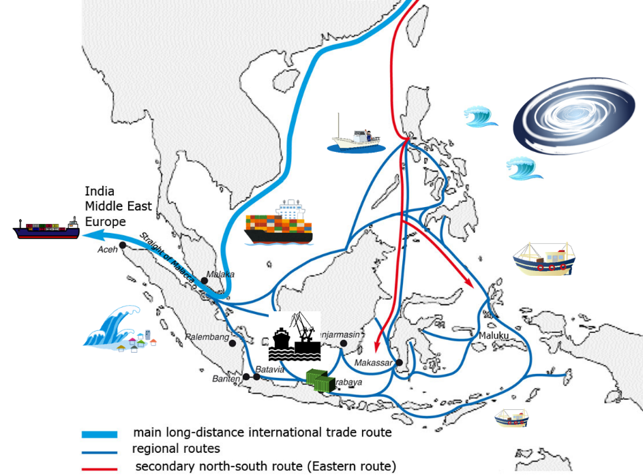
\includegraphics[width = 0.8\linewidth]{Figures/sea_connect.png}
\end{center}
\caption{Improved sea connectivity with SGT}
\label{sea_connect}
\end{figure}

\subsection{Targets}

\begin{enumerate}

\item Smoother and safer transport and logistics in the seas.

\item Reduction of cost/time and marine incidents.

\item Safer and securer industrial activities in the seas.

\item Accident reduction and better control of sea activities.

\item Sustainable management and development of natural resources.

\item Control of natural resource development and conservation of ecosystems.

\end{enumerate}

\subsection{Actions}

\begin{enumerate}

\item Develop marine weather forecast and application center

	\begin{enumerate}
	\item More accurate and integrated marine weather monitoring and forecast

		\begin{enumerate}
		\item Numerical models, data assimilation, satellite data like Himawari
		\end{enumerate}
	
	\item Provide marine data for marine industrial activities such as fishery and aquaculture
	\item Incubate advanced applications for fishery, aquaculture, and environmental management
	\item Model case: IMRO (Indonesia)
	\end{enumerate}

\item Expand world-first advanced positioning services

	\begin{enumerate}
	\item Free and precise, authentication service with QZSS in the seas and ocean
	\item Accelerate social implementation: monitoring and control of fishery, detecting unidentified ships, secure marine logistics, automation of cargo handling etc.
	\end{enumerate}

\item Develop data sharing infrastructure and human resource development facility

	\begin{enumerate}
	\item Marine and land weather, marine logistics, transportation, etc.
	\item Integration of space data and in-situ data
	\item Incubation of data experts serving better data usage and management
	\end{enumerate}

\end{enumerate}


\section{Flagship projects for the development of data sharing infrastructure and related human resources} \label{flagship}

\tab In order to demonstrate the efficiency of SGT in the enhancement of ASEAN connectivity, we present potential flagship projects as well as implementing agencies.

\vspace{0.4 cm}

In particular, beyond the development of data sharing space infrastructure (satellite and ground systems), these projects aim at:

\begin{enumerate}
\item Promoting human resource development for advanced data analysis and usage, including Artificial Intelligence and Internet of Things (IoT) technologies.
\item Demonstrating best practices of data sharing and integration
\end{enumerate}

Concretely, the proposed flagship projects focus on:

\begin{enumerate}

\item Land applications focusing on positioning services, implemented by the GNSS Innovation Center of the Geo-Informatics and Space Technology Development Agency (GISTDA) of Thailand.

\item Marine applications driven by the Institute for Marine Research and Observation (IMRO) of Indonesia.

\item Disaster response and risk management, supervised by the AHA Centre, based in Jakarta, Indonesia.

\item National Space Data Infrastructure and geospatial application centers in each member country.

\end{enumerate}


